\documentclass{beamer}
\usepackage[utf8]{inputenc}

\usetheme{Madrid}
\usecolortheme{default}
\usepackage{amsmath,amssymb,amsfonts,amsthm}
\usepackage{txfonts}
\usepackage{tkz-euclide}
\usepackage{listings}
\usepackage{adjustbox}
\usepackage{array}
\usepackage{tabularx}
\usepackage{gvv}
\usepackage{lmodern}
\usepackage{tikz}
\usepackage{graphicx}

\setbeamertemplate{page number in head/foot}[totalframenumber]

\lstset{
    language=C,
    basicstyle=\ttfamily\small,
    keywordstyle=\color{blue},
    stringstyle=\color{orange},
    commentstyle=\color{green!60!black},
    numbers=left,
    numberstyle=\tiny\color{gray},
    breaklines=true,
    showstringspaces=false,
}

%------------------------------------------------------------
\title{4.5.8}
\date{September 30, 2025}
\author{ADUDOTLA SRIVIDYA - EE25BTECH11006}

\begin{document}

\frame{\titlepage}

\begin{frame}{Question}
The value of $\lambda$ for which the vectors $3i-6j+k$ and $2i-4j+\lambda k$ are parallel is:  
a) $2/3$ \quad b) $3/2$ \quad c) $5/2$ \quad d) $2/5$
\end{frame}


\begin{frame}{Solution}
Given,
\begin{align}
    \myvec{2\\-4\\ \lambda} \text{ is parallel to } \myvec{3\\-6\\1}
\end{align}
If the vectors are parallel, then they are linearly dependent. Hence,
\begin{align}
    \myvec{3 & 2 \\ -6 & -4 \\ 1 & \lambda}\vec{x} = \myvec{0 \\ 0 \\ 0}
\end{align}
To find the condition for non-trivial solutions, perform row reduction on the coefficient matrix:
\begin{align}
\myvec{3 & 2 \\-6 & -4 \\1 & \lambda}
\xrightarrow{R_2 \rightarrow R_2 + 2R_1}
\myvec{3 & 2 \\0 & 0 \\1 & \lambda}
\end{align}
\end{frame}

\begin{frame}{Solution}
    \begin{align}
R_1 \rightarrow \frac{R_1}{3} \implies
\myvec{1 & \frac{2}{3} \\0 & 0 \\1 & \lambda}
\end{align}
\begin{align}
R_3 \rightarrow R_3 - R_1 \implies
\myvec{1 & \frac{2}{3} \\0 & 0 \\0 & \lambda - \frac{2}{3}}
\end{align}
For non-trivial solutions
\begin{align}
    \lambda - \frac{2}{3} = 0
\end{align}
\end{frame}

\begin{frame}{conclusion}
    \begin{align}
    \therefore \lambda = \frac{2}{3}
\end{align}
Hence, the vectors are parallel when $\lambda = \frac{2}{3}$.
\end{frame}

\begin{frame}[fragile]
\frametitle{Python,C,Python+C codes}
codes permalink
\end{frame}

\begin{frame}
\begin{figure}
    \centering
    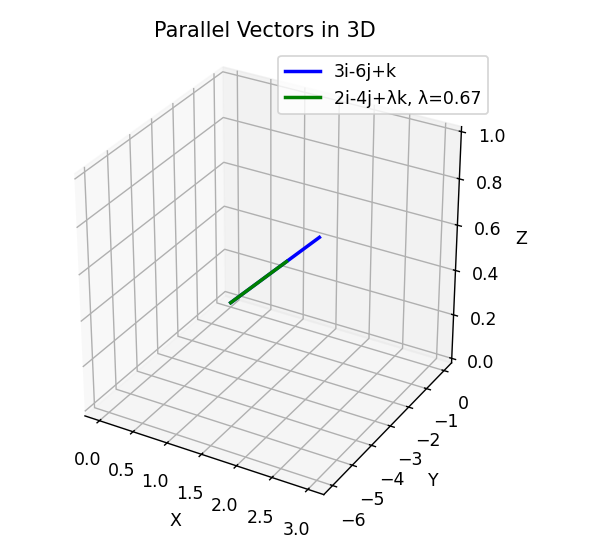
\includegraphics[width=0.5\columnwidth]{figs/fig.png}
    \caption{Vectors $3i-6j+k$ and $2i-4j+\lambda k$ (parallel in 3D)}
    \label{fig:Vectors}
\end{figure}
\end{frame}

\end{document}